\documentclass[letter, 10pts]{article}
\usepackage[monocolor]{../math232/ahsansabit}
\usepackage[]{float}
\usepackage{tikz}
\usepackage{tikz-3dplot}
\usepackage[outline]{contour} % glow around text
\usepackage{xcolor}
\usepackage{pdfpages}
\usepackage{physics}
\usepackage{multicol}
\title{Classical Mechanics : : Homework 09}
\author{Ahmed Saad Sabit, Rice University}
\date{\today}
\newcommand{\hb}{\hbar}
\newcommand{\U}{\uparrow}
\newcommand{\D}{\downarrow}
\usepackage[]{braket}
\begin{document}
\maketitle






























\section*{Problem 01} 
\subsection*{(a)} 
For the first particle in position $\theta = \Omega t$. 
\begin{align*}
\vec{F}_\text{cor} (\theta) &= - 2m \vec{\omega} \times \vec{v}(t) = - 2m \vec{\omega} \times  (\vec{\Omega} \times \vec{R}(t) )\\
&=
- 2 m (\omega \hat{z}) \times  
\left(
\Omega \vec{y} \times 
\left[
R \cos \theta \hat{x} + R \sin \theta \hat{z}
\right]
\right)
\\
&= 
- 2m \omega \hat{z} \times \left(
\Omega R \cos \theta(- \hat{z}) + \Omega R \sin  \theta (\hat{x})
\right)
\\
&= 
2m \omega \hat{z} \times \left(
\Omega R \cos \theta\hat{z} - \Omega R \sin  \theta  \hat{x}
\right)
\\
&= 
2 m \omega \Omega R \sin \theta( \hat{y})
\end{align*}

For the second particle is $\vec{F}_\text{cor}(\theta + \pi )$.  $\vec{F}_\text{cor} = 2 m \omega \Omega R \sin(\omega) \hat{y}$




\begin{figure}[H]
	\centering
	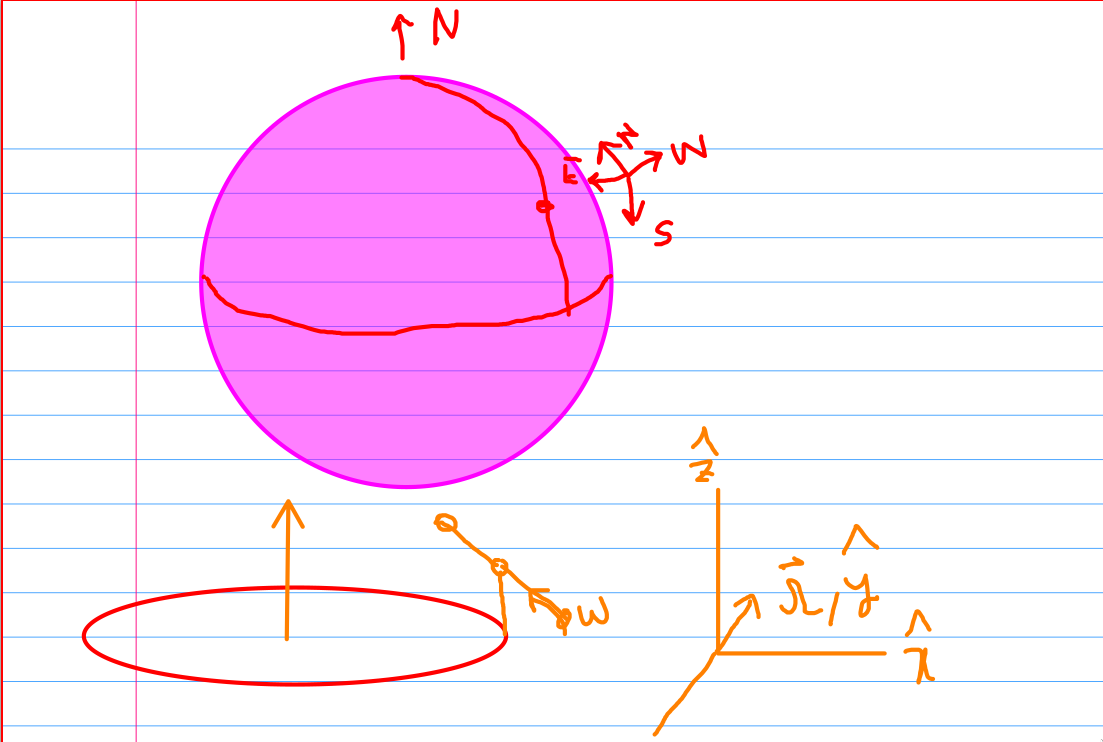
\includegraphics[width=0.8\textwidth]{./ss/9/2.png}
	\caption{./ss/9/2.png}
	\label{fig:-ss-9-2-png}
\end{figure}



\subsection*{(b)} 
\begin{align*}
\vec{\tau} &= 
\vec{R}_1 \times \vec{F}_1 + \vec{R}_2 \times  \vec{F}_2  
\\
&= 
\left(
R \cos \theta \hat{x} + R \sin \theta \hat{z}
\right) \times  ( 2m \omega \Omega R \sin \theta \hat{y})
+ \left(
 -R \cos \theta \hat{x} - R \sin \theta \hat{z}
\right) \times  (- 2m \omega \Omega R \sin \theta \hat{y})
\\
&= 
\left[
	(4 m  \omega \Omega R^2 ) \left(\cos \theta \hat{x} \times \sin \theta \hat{y} + \sin \theta \hat{z} \times  \sin \theta \hat{y}\right)
\right]
\\
&= 
	4 m \omega \Omega R^2  \left(\cos \theta \sin \theta \hat{z}   - \sin ^2 \theta \hat{x}\right)
\end{align*}













\subsection*{(c)} 
\begin{align*}
	\vec{\tau} &= 4 m \omega \Omega R^2 \left(\cos \theta\sin \theta \hat{z} - \sin ^2 \theta \hat{x} \right) \\
	\braket{ \vec{\tau}} 
		   &= \frac{\int_{0}^{T} \mathrm{d} t \,  4 m \omega \Omega R^2 
		   \left(\cos (\Omega t) \sin (\Omega t) \hat{z} - \sin ^2 (\Omega t) \hat{x} \right)}{\int_{0}^{T } \mathrm{d} t }  \\ 
		   &= \frac{\int_{0}^{T} \mathrm{d} t \,  4 m \omega \Omega R^2 
		   \left(\cos (\Omega t) \sin (\Omega t) \hat{z} - \sin ^2 (\Omega t) \hat{x} \right)}{\int_{0}^{T } \mathrm{d} t } 
		   \tag{$T = 2 \pi / \Omega$ } \\ 
&= 
{4 m \omega \Omega R^2} 
\frac{\left[ \hat{z}
\int_{0}^{T} \mathrm{d} t \, \cos(\Omega t) \sin(\Omega t)  - 
\hat{x} \int_{0}^{T} \mathrm{d} t \, \sin ^2 (\Omega t)  
\right]}{2 \pi / \Omega} 
\\
&= 
4 m \omega \Omega R^2 \left(
- \frac{1}{2} \hat{x}
\right)
\\
&= 
-2 m \omega \Omega R^2 
\hat{x}
\\
\end{align*}









\subsection*{(d)} 


New coordinate system where $\hat{y}$ faces the south. And solving for unit mass
\[
\vec{\omega} = \cos(90^{\circ} - \lambda) \hat{z} - \sin(90^{\circ} - \lambda ) \hat{y} 
=
\sin(\lambda) \hat{z} - \cos(\lambda) \hat{y}
\] 
\begin{figure}[H]
	\centering
	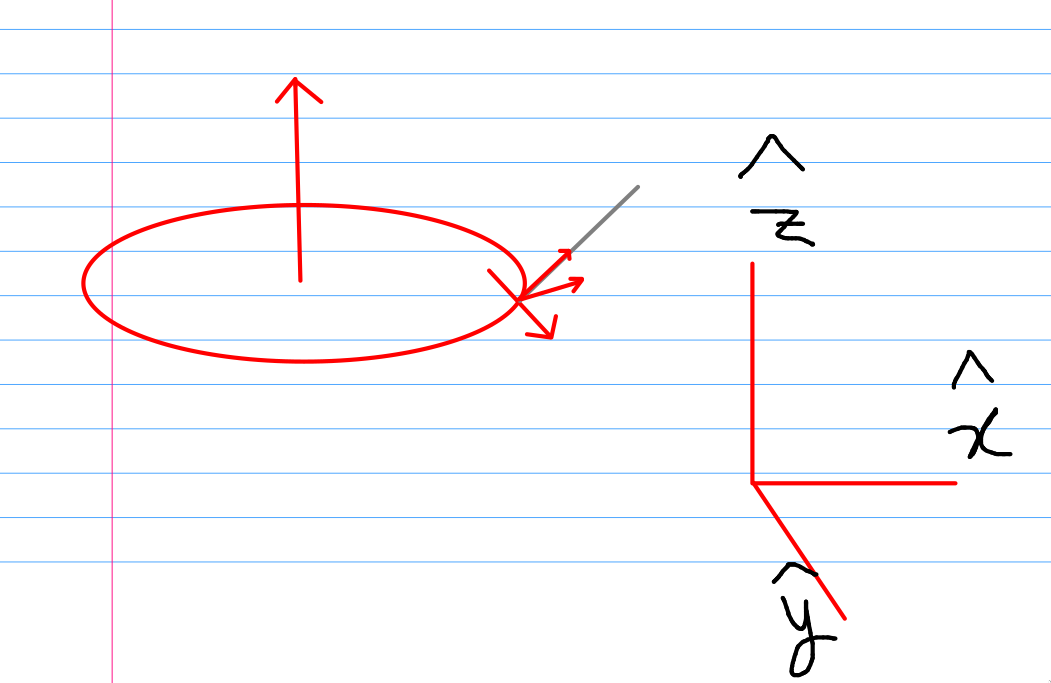
\includegraphics[width=0.8\textwidth]{./ss/9/3.png}
	\caption{.ss/9/3.png}
	\label{fig:-ss-9-3-png}
\end{figure}
Coriolis force
\begin{align*}
\vec{F} &= - 2 \vec{\omega} \times  \vec{v}   \\
&= -2 \omega \left(\sin(\lambda) \hat{z} - \cos (\lambda) \hat{ y}\right)  
\times 
(\vec{\Omega} \times \vec{R} ) \\
&= -2 \omega \left(\sin(\lambda) \hat{z} - \cos (\lambda) \hat{ y}\right)  
\times 
(\Omega \hat{y} \times [R \cos(\theta) \hat{x}  + R \sin (\theta) \hat{z}]) \\
&= -2 \omega (\sin(\lambda) \hat{z} - \cos(\lambda) \hat{y}) 
\times 
\Omega R \left(
\cos (\theta)\hat{z} - \sin(\theta)  \hat{x}
\right)\\
&= -2 \omega \Omega R (\sin(\lambda) \hat{z} - \cos(\lambda) \hat{y}) 
\times 
\left(
\cos (\theta)\hat{z} - \sin(\theta)  \hat{x}
\right)\\
&= 
- 2 \omega \Omega R 
\left[
	\left(
 \cos(\lambda) \cos(\theta) \hat{x}
\right)
+ 
\left(
- 	\sin(\lambda) \sin(\theta) (- \hat{y})  
+ \cos(\lambda) \sin(\theta) (\hat{z})
\right)
\right] \\
&= 
- 2 \omega \Omega R 
\left[
 \cos(\lambda) \cos(\theta) \hat{x}
+ 
	\sin(\lambda) \sin(\theta) \hat{y}  
+ \cos(\lambda) \sin(\theta) \hat{z}
\right] \\
\end{align*}
Torque on single object 
\begin{align*}
\vec{\tau} &=
\vec{R} \times \vec{F} \\
&=
(R \cos(\theta) \hat{x} + R \sin(\theta) \hat{z}) \times  \vec{F} 
\\
&= 
- 2 \omega \Omega R^2 
\left[ -
 \sin \lambda \sin \theta \cos \theta   \hat{z}  
 + 
 \cos\lambda \sin \theta \cos \theta \hat{y} 
 - 
 \cos \lambda \sin \theta \cos \theta \hat{y} 
 + 
 \sin \lambda \sin ^2 \theta \hat{x}
\right]
\\
&= 
2 \omega \Omega R^2 
\left[ 
 \sin \lambda \sin \theta \cos \theta   \hat{z}  
 - 
 \cos\lambda \sin \theta \cos \theta \hat{y} 
 + 
 \cos \lambda \sin \theta \cos \theta \hat{y} 
 - 
 \sin \lambda \sin ^2 \theta \hat{x}
\right]
\\
&= 
2 \omega \Omega R^2 
\left[ 
 \sin \lambda \sin \theta \cos \theta   \hat{z}  
 - 
 \sin \lambda \sin ^2 \theta \hat{x}
\right]
\\
\braket{ \vec{\tau} }&= -  
 \omega \Omega R^2 \sin \lambda  \hat{x}
\\
\end{align*} 

For two particle, symmetrically we will end up with  (considering mass)
\[
\braket{ \vec{\tau}} = - 2 \omega \Omega R^2 \sin \lambda \hat{x}
\] 




\subsection*{(e)} 
The average torque can be measured for various orientations of the rotating axis. Giving between 
$2 \omega \Omega R^2$ to $ 2 \omega \Omega R^2 \sin \lambda $. The maximum gives use the idea of where the west-east line lies and minimum gives idea of  north-south line. 

Then taking care of the direction $- \hat{x}$ we can directly see where the true north is (using similar directions as in the attached figure).









\section*{Problem 02}
\subsection*{(a)}
\begin{align*}
\frac{\mathrm{d} }{\mathrm{d} t} \left(\vec{A} \cdot  \vec{B}\right)_\text{fix} &= 
\left(
\frac{\mathrm{d} \vec{A}}{\mathrm{d} t} \cdot \vec{B}
\right)_\text{fix} + 
\left(
\vec{A} \cdot  \frac{\mathrm{d} \vec{B}}{\mathrm{d} t}
\right)_\text{fix}
\\
\left(
\frac{\mathrm{d} \vec{A}}{\mathrm{d} t} \right)_\text{fix} 
&= 
\left(\frac{\mathrm{d} \vec{A}}{\mathrm{d} t}\right)_\text{rot}+ \vec{\omega} \times \vec{A} \\
\left(
\frac{\mathrm{d} \vec{B}}{\mathrm{d} t} \right)_\text{fix} 
&= 
\left(\frac{\mathrm{d} \vec{B}}{\mathrm{d} t}\right)_\text{rot}+ \vec{\omega} \times \vec{B} \\ 
\\\implies
\frac{\mathrm{d} }{\mathrm{d} t} \left(\vec{A} \cdot  \vec{B}\right)_\text{fix} = 
\left(
\frac{\mathrm{d} \vec{A}}{\mathrm{d} t} \cdot \vec{B}
\right)_\text{fix} + 
\left(
\vec{A} \cdot  \frac{\mathrm{d} \vec{B}}{\mathrm{d} t}
\right)_\text{fix} 
&= \left[
\left(\frac{\mathrm{d} \vec{A}}{\mathrm{d} t}\right)_\text{rot}+ \vec{\omega} \times \vec{A}
\right]\cdot \vec{B}
+\left[
\left(\frac{\mathrm{d} \vec{B}}{\mathrm{d} t}\right)_\text{rot}+ \vec{\omega} \times \vec{B}
\right]\cdot \vec{A}\\
&= 
\left(\frac{\mathrm{d} A}{\mathrm{d} t}\right)_\text{rot} \cdot \vec{B} + 
\left(\frac{\mathrm{d} B}{\mathrm{d} t}\right)_\text{rot} \cdot \vec{A} + 
\left[
	(\vec{\omega} \times \vec{A}) \cdot \vec{B} + (\vec{\omega} \times \vec{B}) \cdot \vec{A}
\right] \tag{check appendix for why third term is zero}
\\
&= 
\left(\frac{\mathrm{d} A}{\mathrm{d} t}\right)_\text{rot} \cdot \vec{B} + 
\left(\frac{\mathrm{d} B}{\mathrm{d} t}\right)_\text{rot} \cdot \vec{A} 
\\
&= 
\frac{\mathrm{d} }{\mathrm{d} t} 
\left(
\vec{A} \cdot \vec{B}\right)_\text{rot}\\
\end{align*}

\subsection*{(b)}
Recycling what we had above, using $\vec{C} = \vec{A} \times \vec{B}$ 
\begin{align*}
	\left( \frac{d\vec{C}}{dt} \right)_{\text{fixed}} &= \left( \left( \frac{d\vec{A}}{dt} \right)_{\text{rotating}} + \vec{\omega} \times \vec{A} \right) \times \vec{B} + \vec{A} \times \left( \left( \frac{d\vec{B}}{dt} \right)_{\text{rotating}} + \vec{\omega} \times \vec{B} \right).
\\
							  &= \left( \frac{d\vec{A}}{dt} \right)_{\text{rotating}} \times \vec{B} + (\vec{\omega} \times \vec{A}) \times \vec{B} + \vec{A} \times \left( \frac{d\vec{B}}{dt} \right)_{\text{rotating}} + \vec{A} \times (\vec{\omega} \times \vec{B})
							  \\ &= 
							  \left[ \left( \frac{d\vec{A}}{dt} \right)_{\text{rotating}} \times \vec{B} + \vec{A} \times \left( \frac{d\vec{B}}{dt} \right)_{\text{rotating}} \right] + \left[ (\vec{\omega} \times \vec{A}) \times \vec{B} + \vec{A} \times (\vec{\omega} \times \vec{B}) \right]
\\
							     &= \left( \frac{d\vec{A}}{dt} \right)_{\text{rotating}} \times \vec{B} + \vec{A} \times \left( \frac{d\vec{B}}{dt} \right)_{\text{rotating}} + \vec{\omega} \times (\vec{A} \times \vec{B}) \tag{check appendix for proof}\\
							     &= \left( \frac{\mathrm{d} }{\mathrm{d} t} \vec{A} \times \vec{B} \right)_{\text{rotating}} + \vec{\omega} \times (\vec{A} \times \vec{B}) \\ 
							     &= 
							     \left(\frac{\mathrm{d} }{\mathrm{d} t} \vec{C}\right)_\text{rotating} + \vec{\omega} \times \vec{C}\\
\end{align*}
So vectors abide by the laws of rotation. 







\section*{Problem 03}
In a  steady rotational frame, intuitively speaking rough - the position dependent force is \emph{Centrifugal Force} and velocity dependent forces are  \emph{Coriolis Force}.  

\subsection*{(a)}
Consider no force of magnetic field now. Then all the fictitious forces where $\vec{r}$ is measured in rotating frame
\[
\vec{F}  = m \ddot{\vec{r}}= \vec{F}_\text{outside } - 2m  \vec{\omega} \times \vec{v} 
- m \vec{\omega} \times (\vec{\omega} \times \vec{r})
\] 
Now including magnetic force
\[
\vec{v}_\text{lab} = \vec{v}_\text{rot} + \vec{\omega}\times \vec{r}
\] 
\[
\vec{F}_\text{B} = - q \vec{v}_\text{lab} \times \vec{B} = -q  (\vec{v}_\text{rot} + \vec{\omega} \times  \vec{r} ) \times \vec{B}
\] 
\[\boxed{
\vec{F}  = m \ddot{\vec{r}}= - 2m  \vec{\omega} \times \vec{v}_\text{rot} 
- m \vec{\omega} \times (\vec{\omega} \times \vec{r})
- q (\vec{v}_\text{rot} + \vec{\omega} \times  \vec{r} )\times \vec{B}
} \] 

\subsection*{(b)} 
Substituting $q = 2 m \omega / B$ yields 
\begin{align*}
	\vec{F} &= - 2m \omega v 
\Biggr[ 
\hat{z} \times \hat{v}
\Biggr]
- m \omega^2 r \Biggr[ \hat{z} \times (\hat{z} \times \hat{r} ) \Biggr]- 
\left(
\frac{2 m \omega}{B}
\right) \Biggr[(vB)\hat{v} \times \hat{z} + (\omega rB)(\hat{z} \times  \hat{r}) \times \hat{z}\Biggr] \\
	&= - 2m \omega v 
\Biggr[ 
\hat{z} \times \hat{v}
\Biggr]
- m \omega^2 r \Biggr[ \hat{z} \times (\hat{z} \times \hat{r} ) \Biggr]- 
2 m \omega v  \Biggr[\hat{v} \times \hat{z} \Biggr]
+
2 m \omega^2 r \Biggr[ \hat{z} \times (\hat{z} \times  \hat{r})\Biggr] \\
	&= 
 m \omega^2 r \Biggr[ \hat{z} \times (\hat{z} \times \hat{r} ) \Biggr] 
\tag{$\vec{A} \times (\vec{B} \times \vec{C}) = (\vec{A} \cdot  \vec{C} ) \vec{B} 
- (\vec{A} \cdot  \vec{B}) \vec{C}$ }
     \\ &=
- m \omega^2 r \Biggr[ (\hat{z}\cdot \hat{z} ) \hat{r} \Biggr]
									\\ &= 
	-							 m \omega^2 \vec{r}
\end{align*}
This leaves us with 
\[
\ddot{\vec{r}} + \omega^2 \vec{r} = 0
\] 
This is a simple harmonic equation, Yippie! Please note that this equation holds in the rotational frame. 




\textbf{Details on shape: } Equilibrium is established at $r = 0$ hence establishing the center of the turntable to be the center. Two component solution 
\begin{align*}
	\ddot{x} + \omega^2 x &= 0  \implies x = x_0 \sin(\omega t + \phi_x)\\ 
	\ddot{y} + \omega^2 y &= 0 \implies y = y_0 \sin(\omega t + \phi_y)\\ 
\end{align*}
This is the very beautiful \emph{Lissayous Curves!}

\begin{figure}[H]
	\centering
	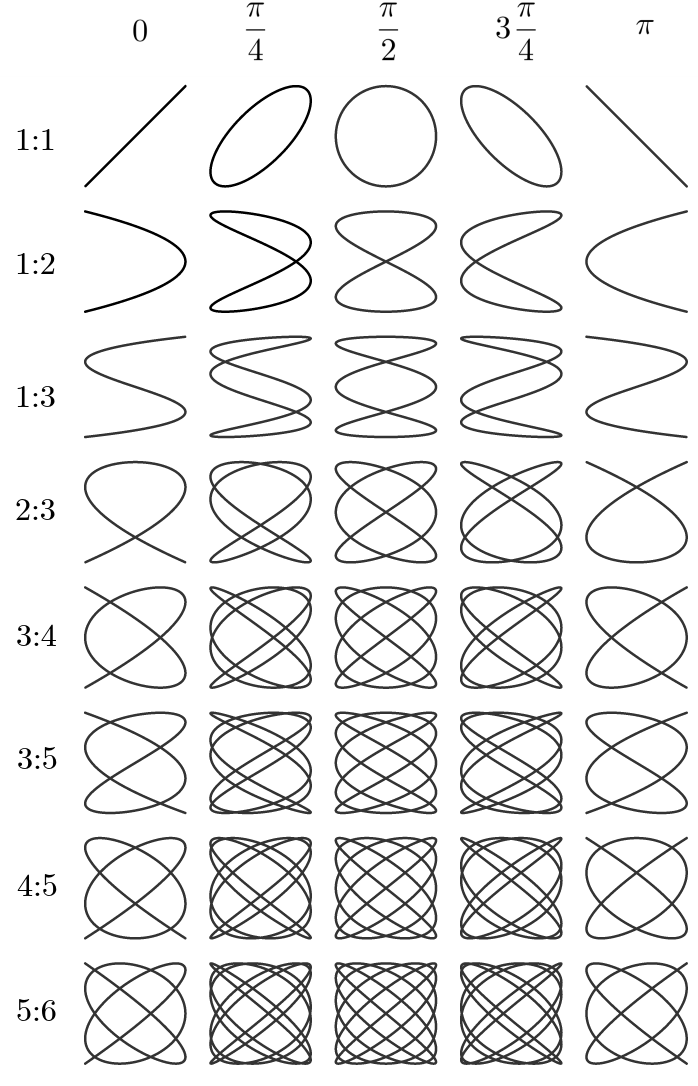
\includegraphics[width=0.8\textwidth]{./ss/9/1.png}
	\caption{Ratio of $x_0:y_0$ versus the phase difference $|\phi_x - \phi_y|$}
	\label{fig:-ss-9-1-png}
\end{figure}



\newpage
\subsection*{(c)}
For half as large $q$ we end up with 
\begin{align*}
	\vec{F} &= - 2m \omega v 
\Biggr[ 
\hat{z} \times \hat{v}
\Biggr]
- m \omega^2 r \Biggr[ \hat{z} \times (\hat{z} \times \hat{r} ) \Biggr]- 
\left(
\frac{ m \omega}{B}
\right) \Biggr[(vB)\hat{v} \times \hat{z} + (\omega rB)(\hat{z} \times  \hat{r}) \times \hat{z}\Biggr]
\\
	&= - 2m \omega v 
\Biggr[ 
\hat{z} \times \hat{v}
\Biggr]
- m \omega^2 r \Biggr[ \hat{z} \times (\hat{z} \times \hat{r} ) \Biggr]- 
\left(
	m \omega v
\right) \Biggr[\hat{v} \times \hat{z} \Biggr] - (m \omega ^2 r) \Biggr[(\hat{z} \times  \hat{r}) \times \hat{z}\Biggr]
\\
	&= - 2m \omega v 
\Biggr[ 
\hat{z} \times \hat{v}
\Biggr]
- m \omega^2 r \Biggr[ \hat{z} \times (\hat{z} \times \hat{r} ) \Biggr] + 
\left(
	m \omega v
\right) \Biggr[\hat{z} \times \hat{v} \Biggr] + (m \omega ^2 r) \Biggr[\hat{z} \times  (\hat{z} \times  \hat{r}) \Biggr]
\\
	&= - 2m \omega v 
\Biggr[ 
\hat{z} \times \hat{v}
\Biggr]
+ \left(
	m \omega v
\right) \Biggr[\hat{z} \times \hat{v} \Biggr] 
     \\ &= 
- m \omega v 
\Biggr[ \hat{z} \times \hat{v}
\Biggr] \\ 
&= 
- m \vec{\omega} \times \vec{v}
\\
\end{align*}

\begin{align*}
	\frac{\mathrm{d} \vec{v}}{\mathrm{d} t} \Biggr|_\text{rot} = -  \vec{\omega} \times  \vec{v}  = \left(\vec{\Omega}\right) \times  \vec{v} 
\end{align*}
So technically in the rotating frame we see the particle itself rotating in $\vec{\Omega} = - \vec{\omega}$
\[
\boxed{
r_0 = \frac{v_0}{\omega}
}
\] %
%
%
%


\section*{Problem 04} 
Total force on any particle
\begin{align*}
\vec{F}/m &= - 2 \vec{\omega} \times \vec{v} +  \vec{g}  \\
&= - 2 (\omega (-\hat{y}) \times v_x \vec{x} + \omega (- \hat{y})\times v_z \hat{z}) -  g \hat{z} \\
&= 2 (\omega \hat{y} \times v_x \hat{x} + \omega \hat{y}\times v_z \hat{z}) -  g \hat{z} \\
&= 2 (\omega v_x (- \hat{z}) + \omega v_z \hat{x}) -  g \hat{z} \\
&= 
\left(- 2 \omega v_x - g \right) \hat{z} + \omega v_z \hat{x}
\\
\ddot{x} &= \omega \dot{z} &\implies \frac{\mathrm{d} ^2 x}{\mathrm{d} t^2} &= \omega \frac{\mathrm{d} z}{\mathrm{d} t}  \\ 
\ddot{z} &= - 2 \omega \dot{x} - g
	 & \implies \frac{\mathrm{d} ^2 z}{\mathrm{d} t^2} &= - 2 \omega \frac{\mathrm{d} x}{\mathrm{d} t} - g \\
\end{align*}

Solve the first differential equation 
\begin{align*}
&\frac{\mathrm{d} ^2x}{\mathrm{d} t^2} = \omega \frac{\mathrm{d} z}{\mathrm{d} t} \\
				      &\text{or, }\frac{\mathrm{d} }{\mathrm{d} t} 
\left(
\frac{\mathrm{d} x}{\mathrm{d} t} 
\right)= 
\frac{\mathrm{d} }{\mathrm{d} t} \left(\omega z + c\right)
				    \\&
\text{or, } 
	\frac{\mathrm{d} x}{\mathrm{d} t} = \omega z + c \\ &
\text{now, } 
\frac{\mathrm{d} ^2 z}{\mathrm{d} t^2} = - 2 \omega \frac{\mathrm{d} x}{\mathrm{d} t} - g
							 \\ &
							\text{or, }
							\frac{\mathrm{d} ^2 z}{\mathrm{d} t^2 } = - 2 \omega^2 z -g + d
\end{align*} 
So setting $z = A \sin(\sqrt{2}  \omega t + \phi) + (K)$ gives us
\[
\frac{\mathrm{d} ^2 z}{\mathrm{d} t^2} = - 2 \omega^2 \left(A \sin (\sqrt{2}  \omega t + \phi)\right)  = -2 \omega^2 (z - K) = - 2 \omega ^2 z + 2 \omega ^2 K \implies K = \frac{-g + d}{2 \omega^2}
\] 

For first order considering $\omega^2 \sim  0$. 
\begin{align*}
&\ddot{x} = \omega \dot{z} &\ddot{z} = - g
\end{align*}

So the deviation 
\begin{align*}
\Delta x &= v_\text{0,x} - \omega v_\text{0,z} t^2 - \frac{1}{3} \omega g t^3   \\
\Delta z &= \Delta z_\text{cor} + \Delta z_g = v_\text{0,z}t - \omega v_\text{o,x} t^2 - \frac{1}{2} g t^2 \\ 
\implies \text{ implying condition } \Delta z = 0 &\implies 
(v_\text{0,z} - \omega v_\text{0,x} t - \frac{1}{2} g t) = 0 \implies t = \frac{v_\text{0,z}}{\omega v_\text{0,x} + g / 2} \\ 
\Delta x &= 
\frac{v_\text{0,x} v_\text{0,z}}{\omega v_\text{0, x} + \frac{1}{2} g }
+
\frac{\omega v_\text{0,z}^3}{(\omega v_\text{0, x} + g / 2 ) ^2 } 
- 
\frac{\omega g v_\text{0,z}^2}{3 (\omega v_\text{0,x} +   g / 2) ^3}
\end{align*}
Numerically solving 
\[
\omega = \sqrt{g / r}  = \frac{1}{30} \text{ rad/s}
\] 
I put the whole thing for $\Delta x$ in a calculator that gives numerically, 
\[
\Delta x = 47 \, \text{m}
\] 




\subsection*{(b)}
There is no sideways ($\hat{y}$) directional deviation for $b$. The coriolis force only acts along the vertical and direction of ball's motion.


\subsection*{(c)} 
There is simply a flip of signs that yields 
\[
\Delta z = 
v_\text{0,z} t + \omega v_\text{0, x} t^2 - \frac{1}{2} g t^2 \implies t = 
v_\text{0,z} \frac{1}{g / 2 - \omega v_\text{0,x}}
\] 
\[
\Delta x = 
\frac{v_\text{0,x} v_\text{0,z}}{ - \omega v_\text{0, x} + \frac{1}{2} g }
+
\frac{\omega v_\text{0,z}^3}{ ( - \omega v_\text{0, x} + g / 2 ) ^2 } 
- 
\frac{\omega g v_\text{0,z}^2}{3 ( - \omega v_\text{0,x} +   g / 2) ^3} = 
\boxed{
57.56 \, \text{m}
}
\] 




\subsection*{(d)} 
\textbf{Effect on height: }
\begin{align*}
a_\text{field}  = \omega^2 r = \text{ numerically } = 10 \text{ m/s}^2
\end{align*}
Error for reaching higher altitude $h \sim 30 \text{ m}$ 
\begin{align*}
\text{error} = 
\frac{
\omega^2 (r - r_0)
}{\omega^2 r} = \text{ numerically } = \frac{1}{300}
\end{align*}
Which is small. \\
\textbf{Horizontal Position:} 
The triangle formed by the horizontal deviation 
\[
z^2 = r_\text{center}^2 - r_\text{end}^2 \sim \text{ numerically } 8999.86 \text{ m}
\] 
The subtended angle 
\[
\cos \theta = \text{ numerically } \implies \theta = 0.32^{\circ}
\] 	
Also negligible. 




















\newpage
\section*{\((\vec{\omega} \times \vec{A}) \cdot \vec{B} = -\vec{A} \cdot (\vec{\omega} \times \vec{B})\)}

\[
\vec{\omega} = (\omega_x, \omega_y, \omega_z), \quad \vec{A} = (A_x, A_y, A_z), \quad \vec{B} = (B_x, B_y, B_z).
\]

\[
\vec{\omega} \times \vec{A} = 
\begin{vmatrix}
\hat{i} & \hat{j} & \hat{k} \\
\omega_x & \omega_y & \omega_z \\
A_x & A_y & A_z
\end{vmatrix}.
\]

\[
\vec{\omega} \times \vec{A} = \big( \omega_y A_z - \omega_z A_y \big)\hat{i} - \big( \omega_x A_z - \omega_z A_x \big)\hat{j} + \big( \omega_x A_y - \omega_y A_x \big)\hat{k}.
\]


\[
(\vec{\omega} \times \vec{A}) \cdot \vec{B} = (\omega_y A_z - \omega_z A_y)B_x + (-(\omega_x A_z - \omega_z A_x))B_y + (\omega_x A_y - \omega_y A_x)B_z.
\]

\[
= \omega_y A_z B_x - \omega_z A_y B_x - \omega_x A_z B_y + \omega_z A_x B_y + \omega_x A_y B_z - \omega_y A_x B_z.
\]

\[
\vec{\omega} \times \vec{B} = 
\begin{vmatrix}
\hat{i} & \hat{j} & \hat{k} \\
\omega_x & \omega_y & \omega_z \\
B_x & B_y & B_z
\end{vmatrix}.
\]

\[
\vec{\omega} \times \vec{B} = \big( \omega_y B_z - \omega_z B_y \big)\hat{i} - \big( \omega_x B_z - \omega_z B_x \big)\hat{j} + \big( \omega_x B_y - \omega_y B_x \big)\hat{k}.
\]


\[
-\vec{A} \cdot (\vec{\omega} \times \vec{B}) = -\left(A_x (\omega_y B_z - \omega_z B_y) + A_y (-(\omega_x B_z - \omega_z B_x)) + A_z (\omega_x B_y - \omega_y B_x)\right).
\]


\[
= \omega_y A_z B_x - \omega_z A_y B_x - \omega_x A_z B_y + \omega_z A_x B_y + \omega_x A_y B_z - \omega_y A_x B_z.
\]

Comparing the expanded expressions for
\[
(\vec{\omega} \times \vec{A}) \cdot \vec{B} \quad \text{and} \quad -\vec{A} \cdot (\vec{\omega} \times \vec{B}),
\]
we see they are identical. Therefore
\[
(\vec{\omega} \times \vec{A}) \cdot \vec{B} = -\vec{A} \cdot (\vec{\omega} \times \vec{B}).
\]


\section*{$(\vec{\omega} \times \vec{A} ) \times  \vec{B} + \vec{A} \times  (\vec{\omega} \times \vec{B})$}

\[
(\vec{\omega} \times \vec{A}) \times \vec{B} = \big((\vec{\omega} \times \vec{A}) \cdot \vec{B}\big) \vec{A} - \big((\vec{\omega} \times \vec{A}) \cdot \vec{A}\big) \vec{B}.
\]


\[
\vec{A} \times (\vec{\omega} \times \vec{B}) = \big(\vec{A} \cdot \vec{B}\big) \vec{\omega} - \big(\vec{A} \cdot \vec{\omega}\big) \vec{B}.
\]

\[
(\vec{\omega} \times \vec{A}) \times \vec{B} + \vec{A} \times (\vec{\omega} \times \vec{B}) = \vec{\omega} \times (\vec{A} \times \vec{B}).
\]
\end{document}
